\documentclass[a4paper, 12pt]{article} % тип документа

%%%Библиотеки
    %\usepackage[warn]{mathtext}	
    \usepackage[T2A]{fontenc}   %Кодировка
    \usepackage[utf8]{inputenc} %Кодировка исходного текста
    \usepackage[english, russian]{babel} %Локализация и переносы
    \usepackage{caption}
    \usepackage{gensymb}
    %\usepackage{listings}
    \usepackage{amsmath, amsfonts, amssymb, amsthm, mathtools}
    \usepackage[warn]{mathtext}
    \usepackage[mathscr]{eucal}
    \usepackage{wasysym}
    \usepackage{graphicx} %Вставка картинок правильная
    \usepackage{pgfplots}
    \usepackage{indentfirst}
    %\usepackage{float}    %Плавающие картинки
    \usepackage{wrapfig}  %Обтекание фигур (таблиц, картинок и прочего)
    \usepackage{fancyhdr} %Загрузим пакет
    \usepackage{lscape}
    %\usepackage{xcolor}
    \usepackage[normalem]{ulem}
    
    \usepackage{titlesec}
    \titlelabel{\thetitle.\quad}

    \usepackage{hyperref}

%%%Конец библиотек

%%%Настройка ссылок
    \hypersetup
    {
        colorlinks = true,
        linkcolor  = blue,
        filecolor  = magenta,
        urlcolor   = blue
    }
%%%Конец настройки ссылок


%%%Настройка колонтитулы
    \pagestyle{fancy}
    \fancyhead{}
    \fancyhead[L]{2.2.3}
    \fancyhead[R]{Глаз Роман, группа Б01-007}
    \fancyfoot[C]{\thepage}
%%%конец настройки колонтитулы



\begin{document}
                        %%%%Начало документа%%%%


%%%Начало титульника
\begin{titlepage}

    \newpage
    \begin{center}
        \normalsize Московский физико-технический институт \\(госудраственный университет)
    \end{center}

    \vspace{6em}

    \begin{center}
        \Large Лабораторная работа по общему курсу физики\\Термодинамика и молекулярная физика
    \end{center}

    \vspace{1em}

    \begin{center}
        \Large \textbf{2.2.3. Измерение теплопроводности воздуха при атомосферном давлении}
    \end{center}

    \vspace{2em}

    \begin{center}
        \large Глаз Роман Сергеевич\\
        Группа Б01-007
    \end{center}

    \vspace{\fill}

    \begin{center}
    Долгопрудный \\2021
    \end{center}
    
\end{titlepage}
%%%Конец Титульника



%%%Настройка оглавления и нумерации страниц
    \thispagestyle{empty}
    \newpage
    \tableofcontents
    \newpage
    \setcounter{page}{1}
%%%Настройка оглавления и нумерации страниц


                    %%%%%%Начало работы с текстом%%%%%%

\textbf{Цель работы:} измерить коэффициент теплопроводности воздуха при атмосферном давлении в зависимости от температуры\\

\textbf{Используемое оборудование:} цилиндрическая колба с натянутой по оси нитью; термостат;
вольтметр и амперметр (цифровые мультиметры); эталонное сопротивление; источник
постоянного напряжения; реостат (или магазин сопротивлений).

\section{Теоретические сведения}

\subsection{Теория}

Для цилиндрически симметричной
установки, в которой поток
тепла направлен
к стенкам цилиндра от нити, расположенной по его
оси, справедлива формула :

$$T_r - T_R = \frac{Q}{2\pi L \chi} \ln \left( \frac{R}{r} \right)$$

Отсюда можно сделать вывод, что разница температур пропорциональна мощности, выделяемой на нити.

$$\chi=\frac{Q}{T_r-T_R}\frac{1}{2\pi L}\ln\left( \frac{R}{r} \right)\eqno(1)$$

Также будут использованы формула Джоуля - Ленца:

$$P=I^2R$$

Связь температуры проводника с его сопротивлением можно описать следующим образом в интервале температур, близких к комнатной температуре:

$$R=R_0(1+\alpha t)$$

\subsection{Схема установки}

\begin{figure}[!h]
    \centering
    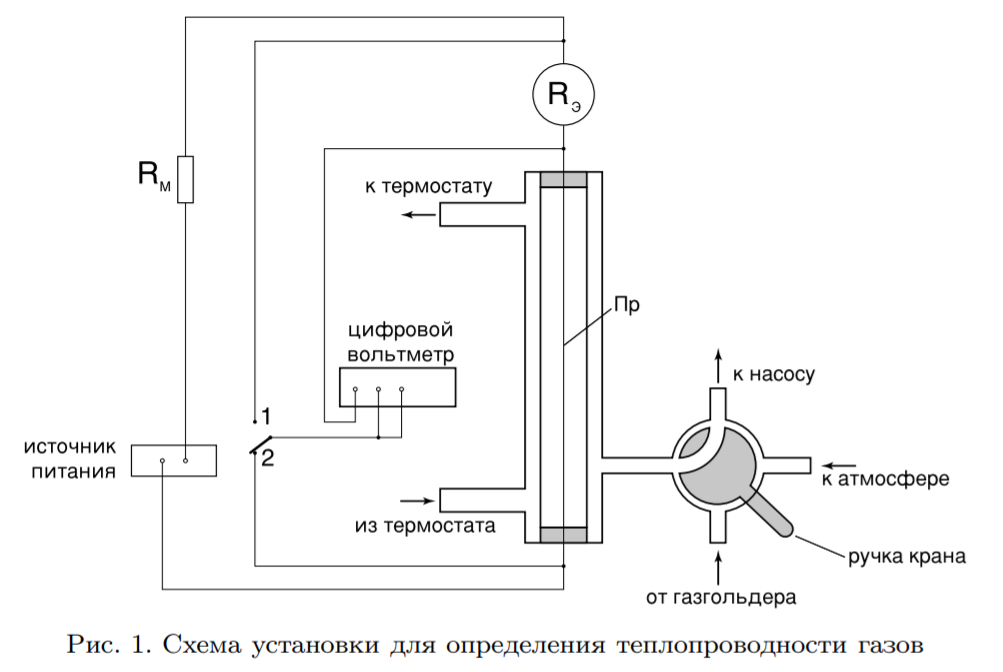
\includegraphics[width = 10 cm]{2.2.3.1.png}
    \caption{Схема установки}
    \label{fig:vac}
\end{figure}

Схема установки изображена на рисунке 1. 

Тонкая нить (никелевая или вольфрамовая проволока) натянута по оси длинной вертикально стоящей медной трубки 1. Через штуцер трубка заполняется исследуемым газом. Нить нагревается электрическим током, ее температура $T_r$ определяется по изменению электрического сопротивления. 

Трубка находится в кожухе, через который пропускается вода из термостата. Температура воды $T_R$ измеряется термометром, помещенным в термостат. Количество теплоты, протекающей через газ, равно (если пренебречь утечками тепла через торцы) количеству теплоты, выделяемому током в нити, и может быть найдено по закону Джоуля—Ленца. 

При этом ток в нити определяется по напряжению на включенном последовательно с ней
эталонном сопротивлении 10 Ом. 

Таким образом, все величины, входящие в правую часть формулы (1), поддаются непосредственному
измерению.


Электрическая часть схемы состоит из источника питания и подключенных к нему последовательно соединенных нити, эталонного
сопротивления 10 Ом и магазина сопротивлений $R_M$, служащего для
точной установки тока через нить. Цифровой вольтметр может подключаться как к нити, так и к эталонному сопротивлению, измеряя
таким образом напряжение на нити и ток через нее.

\subsection{Методика измерений}

Принципиально неустранимая систематическая
ошибка измерения температуры с помощью термометра сопротивления возникает из-за необходимости пропускать через резистор (нить) измерительный ток. Чем этот ток выше, тем с большей точностью будет измерен как он сам, так и напряжение. Однако при этом квадратично возрастает выделяющаяся на
резисторе мощность $Q = I^2 R$. 

Следовательно, температура резистора
становится выше, чем у объекта, температуру которого надо измерить. Измерения же при малых токах не дают достаточной точности (в частности, из-за
существенного вклада термоэлектрических явлений в проводниках и контактах). Эта проблема решается построением нагрузочной кривой — зависимости измеряемого сопротивления $R$ от выделяющейся в нём мощности $R(Q)$, с последующей экстраполяцией к нулевой мощности $Q \rightarrow 0$ для определения сопротивления $R_0 = R(0)$, при котором его температура равна температуре измеряемого объекта. 

Кроме того, в данной работе измерение нагрузочных кривых позволяет в ходе эксперимента получить температурную зависимость сопротивления нити, так как при $Q \rightarrow 0$ температура нити равна температуре
термостата $(T \approx T_0)$.

\section{Ход работы}

\subsection{Снятие данных}

Определим параметры экспериментальной установки:
     
\[L    = 347   \; \text{мм} \]
\[2r = 0,055 \; \text{мм} \]
\[2R = 10    \; \text{мм} \]
\[R_0  = 10    \; \text{Ом} \]        
     
Проведём измерения зависимости падения напряжений от температуры молибденовой нити. Для этого будем устанавливать с помощью магазина напряжений различные напряжения в цепи в интервале от 0,1 до 1,5 В и затем переносить штекер от вольтметра на прибор для измерения теплопроводности. Зависимость снимем для различных температур в интервале от комнатной температуры до 60 градусов по Цельсию. Результаты измерений занесём в таблицу.
     
Сопротивление нити рассчитывается по формуле $R_H = R_0 \frac{U_H}{U_0}$. Выделяемая мощность рассчитывается по формуле $Q = \frac{U_H U_0}{R_0}$. Эти значения также занесём в таблицу 1.


\begin{center}
\begin{tabular}{|c|c|c|c|c|c|c|}
\hline
\textbf{$T$ = 21,3 K} & $U_\text{н}$, мВ & $U_\text{э}$, мВ & $R_\text{э}$, Ом & $I$, мА & $R_\text{н}$, Ом & $P_\text{н}$, мкВт \\ \hline
1                     & 131,85           & 91,69           & 10               & 9,169   & 14,37998         & 1208,933         \\ \hline
2                     & 259,4            & 180,22          & 10               & 18,022  & 14,39352         & 4674,907         \\ \hline
3                     & 389,9            & 270,5           & 10               & 27,05   & 14,41405         & 10546,8          \\ \hline
4                     & 521,31           & 360,87          & 10               & 36,087  & 14,44592         & 18812,51         \\ \hline
5                     & 652,07           & 450,29          & 10               & 45,029  & 14,48111         & 29362,06         \\ \hline
6                     & 784,68           & 540,1           & 10               & 54,01   & 14,52842         & 42380,57         \\ \hline
7                     & 920,12           & 630,8           & 10               & 63,08   & 14,58656         & 58041,17         \\ \hline
8                     & 1055             & 720,1           & 10               & 72,01   & 14,65074         & 75970,55         \\ \hline
9                     & 1271,5           & 860,84          & 10               & 86,084  & 14,77046         & 109455,8         \\ \hline
\end{tabular}
\end{center}

\begin{center}
\begin{tabular}{|c|c|c|c|c|c|c|}
\hline
\textbf{$T$ = 30 K} & $U_\text{н}$, мВ & $U_\text{э}$, мВ & $R_\text{э}$, Ом & $I$, мА & $R_\text{н}$, Ом & $P_\text{н}$, мкВт \\ \hline
1                   & 135,54           & 91,51           & 10               & 9,151   & 14,8115          & 1240,327         \\ \hline
2                   & 468,06           & 315,03          & 10               & 31,503  & 14,85763         & 14745,29         \\ \hline
3                   & 652,75           & 437,82          & 10               & 43,782  & 14,9091          & 28578,7          \\ \hline
4                   & 795,8            & 532,14          & 10               & 53,214  & 14,95471         & 42347,7          \\ \hline
5                   & 918,6            & 612,25          & 10               & 61,225  & 15,00367         & 56241,29         \\ \hline
6                   & 1027,2           & 682,96          & 10               & 68,296  & 15,04041         & 70153,65         \\ \hline
7                   & 1128             & 747,02          & 10               & 74,702  & 15,1             & 84263,86         \\ \hline
8                   & 1221,1           & 806,11          & 10               & 80,611  & 15,14806         & 98434,09         \\ \hline
9                   & 1308,6           & 861,09          & 10               & 86,109  & 15,19702         & 112682,2         \\ \hline
\end{tabular}
\end{center}

\begin{center}
\begin{tabular}{|c|c|c|c|c|c|c|}
\hline
\textbf{$T$ = 35 K} & $U_\text{н}$, мВ & $U_\text{э}$, мВ & $R_\text{э}$, Ом & $I$, мА & $R_\text{н}$, Ом & $P_\text{н}$, мкВт \\ \hline
1                   & 137,53           & 91,26           & 10               & 9,126   & 15,07013         & 1255,099         \\ \hline
2                   & 457,44           & 302,7           & 10               & 30,27   & 15,11199         & 13846,71         \\ \hline
3                   & 633,91           & 418,27          & 10               & 41,827  & 15,15552         & 26514,55         \\ \hline
4                   & 772,36           & 508,19          & 10               & 50,819  & 15,19825         & 39250,56         \\ \hline
5                   & 890,8            & 584,44          & 10               & 58,444  & 15,24194         & 52061,92         \\ \hline
6                   & 996,21           & 651,73          & 10               & 65,173  & 15,28562         & 64925,99         \\ \hline
7                   & 1092,8           & 712,87          & 10               & 71,287  & 15,32958         & 77902,43         \\ \hline
8                   & 1182,3           & 769,02          & 10               & 76,902  & 15,37411         & 90921,23         \\ \hline
9                   & 1226,5           & 821,4           & 10               & 82,14   & 15,4188          & 104030,3         \\ \hline
\end{tabular}
\end{center}

\begin{center}
\begin{tabular}{|c|c|c|c|c|c|c|}
\hline
\textbf{$T$ = 40,2 K} & $U_\text{н}$, мВ & $U_\text{э}$, мВ & $R_\text{э}$, Ом & $I$, мА & $R_\text{н}$, Ом & $P_\text{н}$, мкВт \\ \hline
1                     & 139,77           & 91,54           & 10               & 9,154   & 15,26873         & 1279,455         \\ \hline
2                     & 463,67           & 302,71          & 10               & 30,271  & 15,3173          & 14035,75         \\ \hline
3                     & 642,38           & 418,25          & 10               & 41,825  & 15,35876         & 26867,54         \\ \hline
4                     & 782,67           & 508,18          & 10               & 50,818  & 15,40143         & 39773,72         \\ \hline
5                     & 902,59           & 584,43          & 10               & 58,443  & 15,44394         & 52750,07         \\ \hline
6                     & 1009,37          & 651,76          & 10               & 65,176  & 15,48684         & 65786,7          \\ \hline
7                     & 1106,43          & 712,8           & 10               & 71,28   & 15,52231         & 78866,33         \\ \hline
8                     & 1197,6           & 769,08          & 10               & 76,908  & 15,57185         & 92105,02         \\ \hline
9                     & 1282,72          & 821,5           & 10               & 82,15   & 15,61436         & 105375,4         \\ \hline
\end{tabular}
\end{center}

\begin{center}
\begin{tabular}{|c|c|c|c|c|c|c|}
\hline
\textbf{$T$ = 45,5 K} & $U_\text{н}$, мВ & $U_\text{э}$, мВ & $R_\text{э}$, Ом & $I$, мА & $R_\text{н}$, Ом & $P_\text{н}$, мкВт              \\ \hline
1                     & 141,65           & 91,395          & 10               & 9,1395  & 15,49866         & \multicolumn{1}{l|}{1294,61}  \\ \hline
2                     & 465,1            & 299,23          & 10               & 29,923  & 15,54323         & \multicolumn{1}{l|}{13917,19} \\ \hline
3                     & 643,675          & 413,2           & 10               & 41,32   & 15,57781         & 26596,65                      \\ \hline
4                     & 783,99           & 501,94          & 10               & 50,194  & 15,6192          & 39351,59                      \\ \hline
5                     & 903,95           & 576,725         & 10               & 57,6725 & 15,67385         & 52133,06                      \\ \hline
6                     & 1010,585         & 643,537         & 10               & 64,3537 & 15,7036          & 65034,88                      \\ \hline
7                     & 1107,82          & 704,26          & 10               & 70,426  & 15,73027         & \multicolumn{1}{l|}{78019,33} \\ \hline
8                     & 1198,465         & 758,075         & 10               & 75,8075 & 15,80932         & 90852,64                      \\ \hline
9                     & 1289,75          & 814,79          & 10               & 81,479  & 15,82923         & 105087,5                      \\ \hline
\end{tabular}
\end{center}

\begin{center}
\begin{tabular}{|c|c|c|c|c|c|c|}
\hline
\textbf{$T$ = 50,2 K} & $U_\text{н}$, мВ & $U_\text{э}$, мВ & $R_\text{э}$, Ом & $I$, мА & $R_\text{н}$, Ом & $P_\text{н}$, мкВт \\ \hline
1                     & 143,53           & 91,25           & 10               & 9,125   & 15,72932         & 1309,711         \\ \hline
2                     & 466,53           & 295,75          & 10               & 29,575  & 15,77447         & 13797,62         \\ \hline
3                     & 644,97           & 408,15          & 10               & 40,815  & 15,80228         & 26324,45         \\ \hline
4                     & 785,31           & 495,7           & 10               & 49,57   & 15,84245         & 38927,82         \\ \hline
5                     & 905,31           & 569,02          & 10               & 56,902  & 15,90999         & 51513,95         \\ \hline
6                     & 1011,8           & 635,314         & 10               & 63,5314 & 15,92598         & 64281,07         \\ \hline
7                     & 1109,21          & 695,72          & 10               & 69,572  & 15,94334         & 77169,96         \\ \hline
8                     & 1199,33          & 747,07          & 10               & 74,707  & 16,05378         & 89598,35         \\ \hline
9                     & 1296,78          & 808,08          & 10               & 80,808  & 16,04767         & 104790,2         \\ \hline
\end{tabular}
\end{center}

\begin{center}
\begin{tabular}{|c|c|c|c|c|c|c|}
\hline
\textbf{$T$ = 59,3 K} & $U_\text{н}$, мВ & $U_\text{э}$, мВ & $R_\text{э}$, Ом & $I$, мА & $R_\text{н}$, Ом & $P_\text{н}$, мкВт \\ \hline
1                     & 147,56           & 91,27           & 10               & 9,127   & 16,16742         & 1346,78          \\ \hline
2                     & 479,48           & 295,76          & 10               & 29,576  & 16,21179         & 12079,13         \\ \hline
3                     & 663,32           & 408,41          & 10               & 40,841  & 16,24152         & 27090,65         \\ \hline
4                     & 807,29           & 495,21          & 10               & 49,521  & 16,30197         & 39977,81         \\ \hline
5                     & 931,11           & 569,84          & 10               & 56,984  & 16,33985         & 53058,37         \\ \hline
6                     & 1041,18          & 635,63          & 10               & 63,563  & 16,38028         & 66180,52         \\ \hline
7                     & 1141,6           & 695,08          & 10               & 69,508  & 16,42401         & 79350,33         \\ \hline
8                     & 1234,6           & 749,89          & 10               & 74,989  & 16,46375         & 92581,42         \\ \hline
9                     & 1321,9           & 800,88          & 10               & 80,088  & 16,50559         & 105868,3         \\ \hline
\end{tabular}
\end{center}

\subsection{Исследование зависимостей R(P)}

Построим графики нагрузочных прямых и убедимся, что полученные кривые действительно прямые:


\begin{figure}[!h]
    \centering
    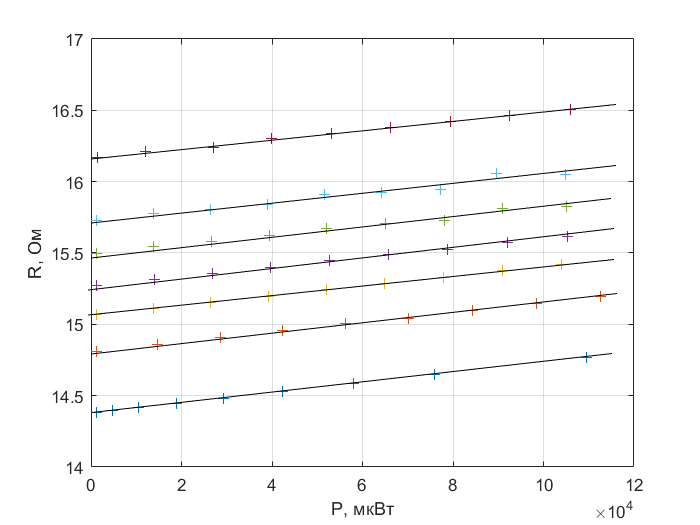
\includegraphics[width = 13 cm]{RQ.png}
    \caption{Зависимости $R(P)$}
    \label{fig:vac}
\end{figure}

Посчтаем с помощью МНК коэффициенты наклона всех прямых, соотнеся с их температурами, также параллельно найдём константы в линейном уравнении зависимостей:

\begin{center}
\begin{tabular}{|c|c|c|c|c|}
\hline
$T$, K & $R_\text{0}$, Ом & $\Delta R_\text{0}$, Ом & $dR/dP$, мОм/Вт & $\Delta \left( dR/dP \right)$, мОм/Вт \\ \hline
21,3   & 14,377           & 0,059                   & 3,445                 & 0,048                                       \\ \hline
30     & 14,808           & 0,031                   & 3,352                 & 0,036                                       \\ \hline
35     & 15,065           & 0,034                   & 3,303                 & 0,035                                       \\ \hline
40,2   & 15,272           & 0,029                   & 3,263                 & 0,033                                       \\ \hline
45,5   & 15,523           & 0,039                   & 3,236                 & 0,038                                       \\ \hline
50,2   & 15,723           & 0,049                   & 3,202                & 0,049                                       \\ \hline
59,3   & 16,167           & 0,041                   & 3,077                 & 0,037                                       \\ \hline
\end{tabular}
\end{center}

\subsection{Получение теплопроводности газа}

Теперь рассмотрим, каким образом зависит начальное значение сопротивления нити от температуры, при которой находилась установка во время измерений:

\begin{figure}[!h]
    \centering
    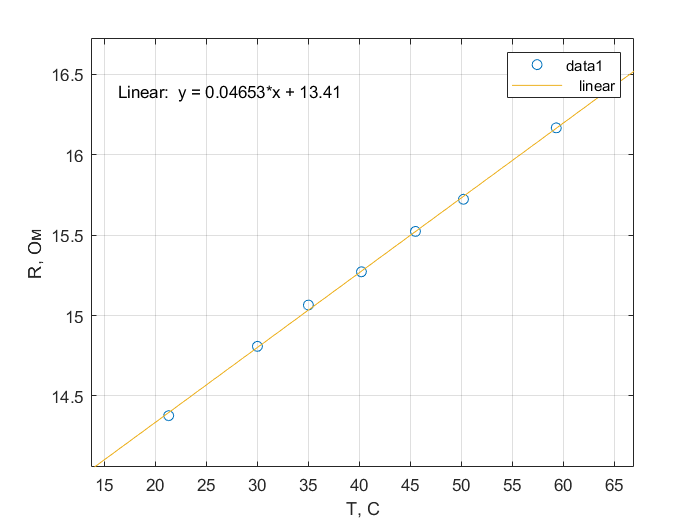
\includegraphics[width = 13 cm]{RT.png}
    \caption{Зависимости $R(T)$}
    \label{fig:vac}
\end{figure}

Так как известны погрешности опреления сопротивлений, можно воспользоваться методом хи-квадрат. Для этого необходимо, чтобы погрешности измерения температуры были меньше, чем сопротивления (гораздо меньше). Для температуры оценим погрешность (взяв максимум): $\sigma_T = 0,1 / 300 = 3,33 \cdot 10^{-4}$, для сопротивлений имеем $\sigma_R = 0,04 / 14 = 2,85 \cdot 10^{-3} \gg \sigma_T$. Значит можно воспоьзоваться критерием Пирсона (хи-квадрат):

\begin{equation}
    \frac{dR}{dT} = 4,53 \cdot 10^{-2} \; \text{Ом/К}
\end{equation}

\begin{equation}
    \Delta \left( \frac{dR}{dT} \right) = 0,098 \cdot 10^{-2} \; \text{Ом/К}
\end{equation}

При этом теперь можем связать мощность, выделяющуюся при протекании тока, с температурой:

\begin{equation}
    \frac{dP}{dT} = \frac{dP dR}{dT dR} = \frac{\frac{dR}{dT}}{\frac{dR}{dP}}
\end{equation}

\begin{center}
\begin{tabular}{|c|c|c|c|c|}
\hline
$T$, K & $dP/dT$, Вт/ К & $\Delta \left( dP/dT \right)$, Вт/К & $\kappa, \; \text{Вт}/(\text{м} \cdot \text{К})$ & $\Delta \kappa, \; \text{Вт}/(\text{м} \cdot \text{К})$ \\ \hline
21,3   & 13,147        & 0,439                               & 29,574 & 1,069                                                  \\ \hline
30     & 13,513         & 0,395                               & 29,831                                           & 1,029 \\ \hline
35     & 13,714         & 0,407                               & 30,275                                           & 1,041                                          \\ \hline
40,2   & 13,882         & 0,401                               & 30,645 & 1,036                                                  \\ \hline
45,5   & 14,000         & 0,409                               & 30,906                                           & 1,045                                                  \\ \hline
50,2   & 14,147        & 0,442                               & 31,231 & 1,073                                                  \\ \hline
59,3   & 14,719         & 0,436                               & 32,493                                           & 1,065                                                  \\ \hline
\end{tabular}
\end{center}

Погрешности для найденным значений теплопроводности найдём из формулы для косвенных погрешностей:

\begin{equation}
    \Delta \kappa = \kappa \sqrt{ \left( \frac{\sigma_{dP/dT}}{dP/dT} \right)^2 + \left( \frac{\sigma_{L}}{L} \right)^2 + \left( \frac{\sigma_{r}}{r} \right)^2 + \left( \frac{\sigma_{R}}{R} \right)^2}
\end{equation}

Из таблицы видно. что последняя точка явно выбивается из тенденции возрастания коэффициента теплопроводности, поэтому далее не будем её учитывать.

Построим график зависимости теплопроводности от температуры (кривая, аппроксимирующая зависимость полиномом, приведена только для наглядности):

\begin{figure}[!h]
    \centering
    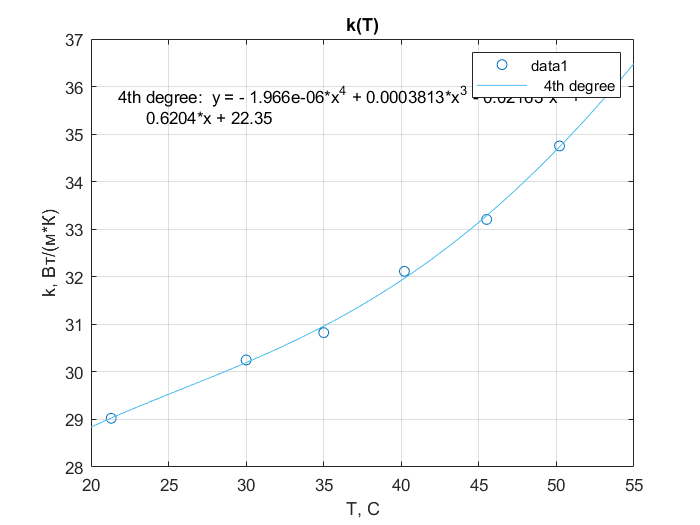
\includegraphics[width = 13 cm]{KT.png}
    \caption{Зависимости $\kappa (T)$}
    \label{fig:vac}
\end{figure}

Предполагая, что зависимость теплопроводности от температуры степенная, прологарифмируем полученную зависимость (заметим, что на данном этапе уже потеряна большая разница в погрешностях для различныъ температур из-за наличия косвенных измерений, которые в большей степени повлияли на погрешность, а значит при логарифмировании можно считать погрешности практически эквивалентными и целесообразно воспользоваться МНК):

\begin{center}
\begin{tabular}{|c|c|c|}
\hline
$T$, K & $ln(T)$ & $ln(\kappa)$ \\ \hline
21,3   & 5,6851  & 3,3875       \\ \hline
30     & 5,7043  & 3,3955       \\ \hline
35     & 5,7208  & 3,4103       \\ \hline
40,2   & 5,7473  & 3,4225       \\ \hline
45,5   & 5,7641  & 3,4310       \\ \hline
50,2   & 5,7797  & 3,4414      \\ \hline
\end{tabular}
\end{center}

\begin{figure}[!h]
    \centering
    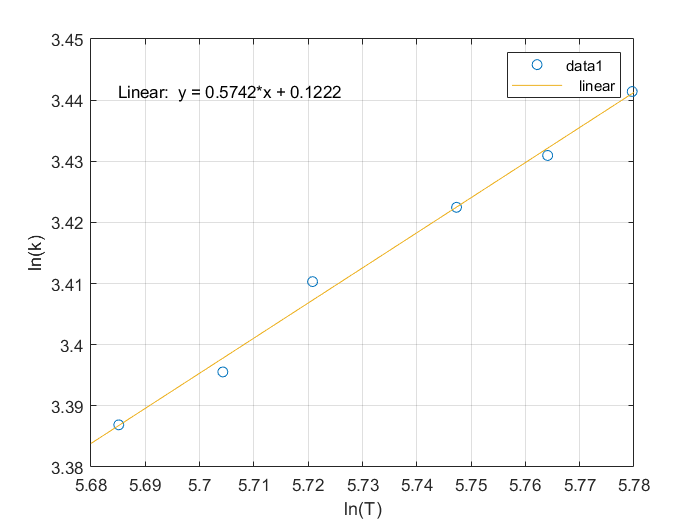
\includegraphics[width = 13 cm]{lnKT.png}
    \caption{Зависимости $ln(k)(ln(T))$}
    \label{fig:vac}
\end{figure}


Имеем по МНК:

\begin{equation}
    \kappa = C \cdot T^{\beta}, \;  \text{где } \beta = 0,574, \; \Delta \beta = 0,037
\end{equation}

Заметим, что полученное значение сохраняет теоретическую направленность, что коэффициент выходит меньше единицы. Более того, по значение он почти совпадает с теоретическим значением (0,5). 


\section{Заключение}

\begin{enumerate}

    \item В ходе работы была экспериментально определена теплопроводность воздуха при различных температурах, обнаружена линейная зависимость этих величин.
    \item Были оценены погрешности измерения зависимости сопротивления молибденовой нити и мощности, выделяющейся на ней. Основной вклад в величину погрешности вносит относительная погрешность измерения напряжения на эталонном сопротивлении: 0,1 В при классе точности прибора вольтметра 0,01 В.
    \item Экспериментально было определено значение температурного коэффициента молибдена: значение, которое можно получить из снятых измерений, равно $\alpha = 0.00453 \pm 0.00038$ $K^{-1}$, в то время как табличное значение  $\alpha = 0.004579$ $K^{-1}$.
    \item Был определён характер зависимости коэффициента теплопроводности газа от температуры. Полученная зависимость почти сошлась в выведенной теоретически ($\kappa = AT^{1/2} $). Различие может быть связано с погрешностями при проведении эксперимента (методическими).
    
\end{enumerate}

\section{Список используемой литературы}

$\bullet$ Гладун А. Д. Лабораторный практикум по общей физике. Термодинамика и молекулярная физика\\

$\bullet$ \href{https://mipt.ru/education/chair/physics/S_II/lab/}{Описание лабораторных работ на кафедре общей физики МФТИ}

\end{document}